\chapter{Linear Collider Concepts}
\section{Luminosity}
Luminosity, $L$, is proportional to the number of collisions that are produced when two beams cross each other. The expression that relates luminosity, cross section $\sigma$ and the number of events produced $R$ is given by,
\begin{equation}
 R=L\sigma
\end{equation}
Luminosity will depend on the bunch population 	$N$ (assuming an equal number of particles for both beams) and their density distribution within the bunches 
% \section{Optics}
\section{Beam Delivery System (BDS)}
After the acceleration, in the Beam Delivery System (BDS) the beam needs to be focused and higher order aberrations must be compensated to obtain nanometer beam size. 
\section{Final Focus Sections (FFS)}
\section{Overview of FFS effects}
\subsection{Beamstrahlung}
\subsection{Hourglass effect}
Since the $\beta$-functions have their minimum at the IP and increase with the longitudinal distance, to consider the beam size constant along the whole collision length is some cases is not a good approximation. In a low-$\beta$ region 
\subsection{Crossing angle}
\subsection{Chromaticity}
relative path 
\begin{figure}[!hbt]
\centering
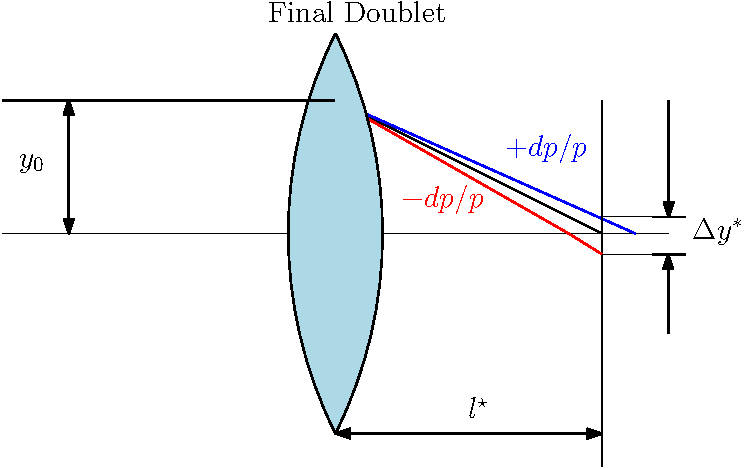
\includegraphics[scale=0.5]{chromaticity.pdf}\caption{Chromaticity.}\label{f:chrom}
\end{figure}
\subsection{Tuning}
When considering imperfections, the machine performance decreases dramatically, typically, the beam size increases and luminosity drops substantially about 6 orders of magnitud. The tuning is the procedure which brings the system performance to its design values. Since the initial errors are unknown, the tuning requires a statistical study. Usually more than 100 machines with randomly distributed errors are considered in computer simulations. The simulated tuning reproduces a realistic tuning procedure in a machine \cite{GarciaMorales:1982827,Minty:629879}.\par
